%% LyX 2.3.2-2 created this file.  For more info, see http://www.lyx.org/.
%% Do not edit unless you really know what you are doing.
\documentclass[UTF8]{ctexart}
\usepackage{amsmath}
\usepackage{fontspec}
\usepackage{geometry}
\geometry{verbose,tmargin=2.6cm,bmargin=2.6cm,lmargin=3.6cm,rmargin=3.6cm}
\usepackage{float}
\usepackage{graphicx}
\usepackage{setspace}
\onehalfspacing
\usepackage[unicode=true,pdfusetitle,
 bookmarks=true,bookmarksnumbered=false,bookmarksopen=false,
 breaklinks=false,pdfborder={0 0 0},pdfborderstyle={},backref=false,colorlinks=false]
 {hyperref}

\makeatletter

%%%%%%%%%%%%%%%%%%%%%%%%%%%%%% LyX specific LaTeX commands.
\newcommand{\lyxmathsym}[1]{\ifmmode\begingroup\def\b@ld{bold}
  \text{\ifx\math@version\b@ld\bfseries\fi#1}\endgroup\else#1\fi}

%% A simple dot to overcome graphicx limitations
\newcommand{\lyxdot}{.}

\floatstyle{ruled}
\newfloat{algorithm}{tbp}{loa}
\providecommand{\algorithmname}{算法}
\floatname{algorithm}{\protect\algorithmname}

%%%%%%%%%%%%%%%%%%%%%%%%%%%%%% User specified LaTeX commands.
\usepackage{listings}
\usepackage{xcolor}
\lstset{ 
    language=verilog,
    backgroundcolor=\color{blue!1},
    basicstyle=\small\ttfamily,
    breaklines=true,
    numbers=left,
    numberstyle=\tiny\menlo,
    showstringspaces=false,
    keywordstyle=\color{blue!60},
    commentstyle=\color{red!50!green!50!blue!50}, 
    stringstyle=\color{purple!60},
    frame=shadowbox,
    rulesepcolor=\color{ red!20!green!20!blue!20},
    escapeinside=``,
    xleftmargin=1em,
    xrightmargin=1em,
    aboveskip=1em,
    framexleftmargin=2em
}
\usepackage{hyperref}
\usepackage{movie15}

\@ifundefined{showcaptionsetup}{}{%
 \PassOptionsToPackage{caption=false}{subfig}}
\usepackage{subfig}
\makeatother

\begin{document}
\title{基于深度学习的字体编码文档水印技术作品报告}

\maketitle
\newpage{}
\begin{center}
\textbf{填写说明}
\par\end{center}
\begin{enumerate}
\item 所有参赛项目必须为一个基本完整的设计。作品报告书旨在能够清晰准确地阐述(或图示)该参赛队的参赛项目(或方案)。
\item 作品报告采用A4纸撰写。除标题外,所有内容必需为宋体、小四号字、1.5倍行距。
\item 作品报告中各项目说明文字部分仅供参考,作品报告书撰写完毕后,请删除所有说明文字。(本页不删除)
\item 作品报告模板里已经列的内容仅供参考,作者可以在此基础上增加内容或对文档结构进行微调。
\item 为保证网评的公平、公正,作品报告中应避免出现作者所在学校、院系和指导教师等泄露身份的信息。
\end{enumerate}
\newpage{}

\tableofcontents{}

\newpage{}
\begin{abstract}
(请简要说明创作本作品之动机、功能、特性、创新处、实用性)

文档水印技术的重要性。

针对文档溯源问题,本作品提出在中文文档中进行高精度、高鲁棒性文档水印的关键技术,并实现了一个原型系统来演示其效果。演示系统基于屏摄文档,但可以扩展到其他形式的文档,具有普遍应用的潜力。
\end{abstract}
\newpage{}

\part{作品概述}

(建议包括:背景分析、相关工作、特色描述及应用前景分析等)

\section{研究背景}

随着信息化时代的到来,电子文档成为日常办公文档的主要形式。目前对于重要文件的保护主要还是依靠传统的方案,通过加密,访问控制,身份认证等手段对电子文档进行保护。但是随着智能手机的普及,在将一些文字内容在屏幕上进行投射展示时,因为手机拍摄导致信息泄漏的情况越来越频繁。传统的解决方案是在文档中嵌入水印添加额外信息保证文档可溯源,保护文档知识产权。但是传统的嵌入水印技术在经过屏摄这一过程后,嵌入的信息会大量丢失,完全无法恢复原始信息。

针对文档的抗屏摄水印技术可以将屏摄的时间地点和所有权版本等信息嵌入到文档中。在文件因拍照泄漏后,可以通过提取水印信息找到泄漏的具体时间地点,起到文档溯源的作用。因此,研究此项技术有着迫切的需求与极大的价值。

利用象形文字的字体进行编码,即使经过了屏摄处理之后,象形文字的字体信息仍然可以保留。为了达到隐写信息的目标,文档应用肉眼不可识别的不同字体构成。准确识别本身非常相近的字体是一个难点,特别是在经过屏摄处理之后的图像保留的区分信息更会减少。这一问题难以使用传统的算法进行解决,因此本作品使用深度学习技术构建了学习能力足够强的神经网络,同时拍摄了大量的训练数据来增强网络的泛化能力。结合识别字体的神经网络和带有纠错能力的编码方案,本系统实现的字体编码文档水印技术可以大幅增强抗屏摄能力。

\section{相关工作}

我们的工作基于Chang Xiao 2018\cite{xiao2018fontcode}:利用英文字体的细微差别在文档中进行信息隐藏。然而,我们的工作难度更大,体现在以下三个方面。第一个方面,Chang
Xiao2018\cite{xiao2018fontcode}是基于英文字母的字体差别进行的信息隐藏。英文字母只有26个,然而我们进行的中文字体隐写需要识别的常用字就有3000及以上。这对我们的神经网络识别能力提出了非常高的要求,在采集训练集时数据量也会大大增加。第二个方面,中文字体和英文在形状上有很大不同。考虑到中文字体有偏旁部首(整个字体不是连通的),分割取字也变得更有难度。第三个方面,我们是对屏幕上显示的文档拍照进行识别。在屏摄过程中产生的失真、摩尔纹、噪点等都会大大影响神经网络模型的识别率。

\paragraph{编码字体的选择}

我们的字体编码工作需要选择字形相似且不易被人察觉出差异的字体。目前有很多种选择字体的方法。进来,众包技术\cite{o2014exploratory}以及提取相似度\cite{loviscach2010universe}经常被使用。考虑到我们的系统只需要验证方案的可行性。我们在之前的已有的技术上做了融合和裁减,只选择部分可行字体进行实现,并使用众包技术验证字体的不可区分性。

\paragraph*{支持拍照后的字体识别}

由于拍照会导致原本文档中的信息流失,大部分的隐写技术在拍照后都会变得不可靠甚至完全无法使用。Jiren Zhu 2018\cite{zhu2018hidden}是一项针对拍照后提取图像中隐写信息的工作,这与我们拍照后识别字体具有很大的相似度。但是,图像隐写与字体隐写还是有本质的差异。图像隐写可以将隐写信息置于整张图片中(大部分是一个规则的矩形),隐写面积更大,也更易识别隐写区域。我们的字体隐写识别别区域仅在字体本身,隐写面积很小,每个字体的识别区域也不同。

之前也有很多识别图片中字体的工作,如Carlos Avilés-Cruz 2015\cite{aviles2005high}——使用静态方法提取字体特征进行识别。进来,神经网络与深度学习技术崛起兴盛,使用神经网络识别字体的技术越来越多,而且效果都非常好。Chen
2014\cite{chen2014large}中就提出了一种规模可变的监督学习方法。随后Wang 2015\cite{wang2015deepfont}提出使用CNN识别字体的方案。我们的识别方法也运用了神经网络,并将CNN作为核心的一环。最终搭建的网络模型使用了一种效果非常好的图片分类模型
——He 2016\cite{he2016deep}。我们调整了模型的部分细节和参数以适应于整个任务。

\paragraph{在文档中隐写信息}

我们的工作与隐写技术相关。各种载体上(图像、光照、音频、视频)的隐写技术都被研究了多年。但是基于文档中文字的隐写更有挑战性,目前较为成熟的隐写方案也比较少。我们在这里列出几种现有的文档中隐写信息的方案。

第一种方案是cover text generation CTG,wayner 1992 2009\cite{wayner1992mimic}\cite{wayner2009disappearing}。这种方案生成一种语法和句法上非常自然的文档,在词句之中隐藏信息。这种方案的缺点也是非常明显的——它不能给定文档进行隐写。

第二种方案是黄兴 2013\cite{黄兴2013抗打印扫描的文本数字水印技术研究},将字体边缘的像素翻转来进行编码。这种方案的缺点在于信息流失的可能性太大,特别是在屏摄后能识别出隐写信息的概率非常小。而且,如果采用这种方法,对所有格式文档适应的成本也非常高。

第三种方案利用了文档格式上的特征,例如改变文字大小、颜色、下划线等 TODO

\paragraph{隐写信息的编码解码}

由于编码所采用的字体差别非常小,在屏摄过后字体差别会更小,神经网会有一定概率识别出错。在这种情况下,使用纠错码是非常有必要的。我们使用了BCH编码\cite{bose1960class}。该编码算法能允许48比特内出5比特错。只要我们的神经网络识别错误率在BCH编码允许内,就能完整的还原隐写的信息。最终,我们的网络确实达到了要求,能够还原出隐写信息。

\section{特色描述\label{sec:=007279=008272=0063CF=008FF0}}

\subsection{产品特色}

本作品实现了抗屏摄的文档字体水印技术。由于智能手机的普及,抗屏射已经成为水印技术的重大难点。传统水印处理过的文档在通过手机拍摄这一处理后,水印的大部分特征已经丢失,无法还原出正确的水印信息。本作品创新性地使用肉眼难以分辨的字体作为信息载体在文档中加入水印,通过深度学习的技术来识别出不同字体的特征,从而实现字体编码。本作品的水印方案能够很好的解决屏射后信息丢失的问题,目前的系统可以非常好的从手机拍摄的水印文档的图片中还原出原始信息。

\subsection{核心算法特色}

本作品使用深度学习技术,结合自行拍照、矫正、切割字符制作的数据集进行模型训练,在识别屏射后的字体上取得了很高的训练精度。在准确识别字体的基础上,根据测试得到的误码率选择了合适的纠错编码方案,达到了准确恢复水印信息的效果。为了演示字体识别的准确性,本作品设定了一个易于处理的文档布局方式,并基于该布局方式实现了自动文档识别和准确的文字分割。目前的信息提取率已经做到了92.5\%,结合BCH纠错码信息恢复准确度可以达到99\%以上。
\begin{enumerate}
\item 因为文档水印的主要需要保障信息的完整性,所以必须选择有很强的纠错功能的编码方案。从而保证在有限的识别字体的准确度的情况下,仍然可以非常好的保证水印信息不会丢失。
\item 文档在经过手机拍摄后不可避免的会出现各种噪点、模糊的情况。以及因为拍摄距离和拍摄角度等影响,拍摄过后的文档文字上还会出现摩尔纹或产生畸变。我们设计并且实现了畸变矫正算法,并且在采集训练数据的过程中制造了各种环境情况,保证了神经网络的泛化能力足够抵抗大多数的屏射情况。
\item 采用人眼很难分辨的字体编码信息,需要网络有足够学习能力提取出不同字体的特征。我们设计并且不断改善网络的结构,针对于大量的数据集不断训练增强模型的分类能力。图片的背景颜色和环境因素都会对神经网络的识别特征造成干扰,我们设计并实现了减少背景颜色和噪点等因素影响的数据预处理方案。
\end{enumerate}

\section{应用前景分析}

\subsection{文档溯源}

在政府及企业部门中,文档的保密性始终是一个重要的问题,机密文档的泄露将威胁企业及国家的安全,带来极大的风险。

首先要从源头避免文档的泄露,对于重要文件的打印,可以采用限制打印、复印次数,或指定专人负责,以进行保密,打印文档时需要经过批准,审批,登记等步骤,并定期对纸质文档进行销毁或归档处理。对于重要的电子文档往往采用访问控制、身份认证等手段进行保护。

尽管有这些保密措施,但在用户获得文档的副本后,其去向就难以控制,信息泄露的风险加大。当文档泄露后,如果能定位文档泄露源头并对其进行管控、跟踪和追责,就可以及时避免更大的损失。因此,对文档进行可溯源的发布有着迫切的需求与极大的价值。

要使文档可溯源,就要向其中加入水印。针对文本文档的抗打印扫描的数字文本水印技术能够将打印负责人的身份信息作为水印嵌入到将打印的纸质文件中,在文件泄露被捕获后通过提取水印信息即可对纸质文件泄密源头进行管控追踪。因此,研究此项技术有着迫切的需求与极大的价值。

\subsection{信息推送}

在商业宣传和海报制作中,设计者往往会在其作品上添加二维码来方便用户获取详细信息,但是二维码形态相对固定,对作品的整体效果有一定的影响,因此在实际使用时人们往往会为其加上多样的形态进行美化。如果能够在艺术宣传作品的文字中直接嵌入网站链接等信息,就能够免去二维码,进一步减小对设计者的约束。

\newpage{}

\part{作品设计与实现}

(建议包括系统方案、实现原理、硬件框图、软件流程、功能、指标等)

\section{系统设计}

在核心算法的基础上,我们设计和实现了一个简单的原型系统用以展示我们的文档水印技术。

\subsection{使用流程}

\subsubsection{文档发布}

当用户需要发布一份带水印的文档时,首先将文档原文和水印信息提交至本系统,由本系统生成带有水印的文档,然后用户获取该文档,进行后续的处理和使用。

\begin{figure}[H]
\centering{}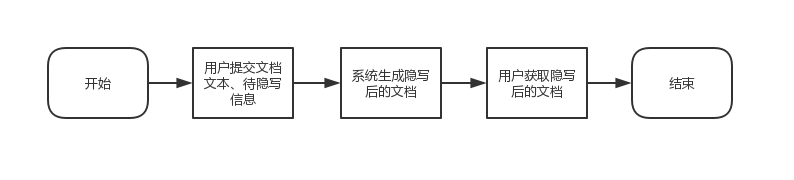
\includegraphics[width=14cm]{figures/doc-pub-steps}\caption{文档发布流程图}
\end{figure}


\subsubsection{信息提取}

当用户需要从带有水印的文档中恢复信息时,首先对文档进行拍照或扫描以得到电子版本,然后将该电子版本提交至系统,系统分析出水印内容后反馈呈现给用户。

\begin{figure}[H]
\centering{}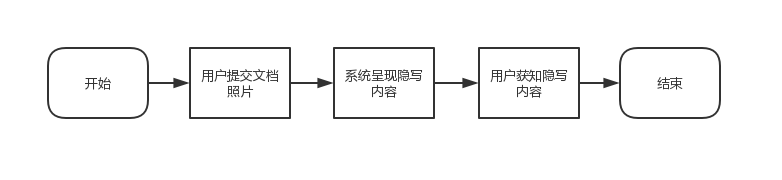
\includegraphics[width=14cm]{figures/doc-read}\caption{信息提取流程图}
\end{figure}


\subsection{系统架构}

我们的原型系统使用服务端-客户端架构。如下图所示:

\begin{figure}[H]
\centering{}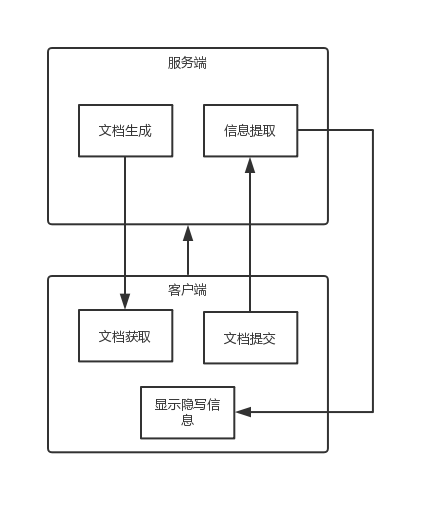
\includegraphics[width=10cm]{figures/sys-arch}\caption{系统架构图}
\end{figure}


\paragraph{服务端}

文档水印和提取的核心算法部署在服务端,此外,服务端含有图片文档切割、矫正、字符切分算法以及与客户端通信的功能。

\paragraph{客户端}

向用户提供方便地与系统进行交互的接口,用户通过客户端获取文档、从文档中读取水印信息。客户端可以以多种形式实现,包括 Web 页面、微信小程序、手机
App 等,我们的演示系统中以微信小程序的形式提供客户端。

\section{功能模块}

\subsection{文档生成模块}

\begin{figure}[H]
\begin{centering}
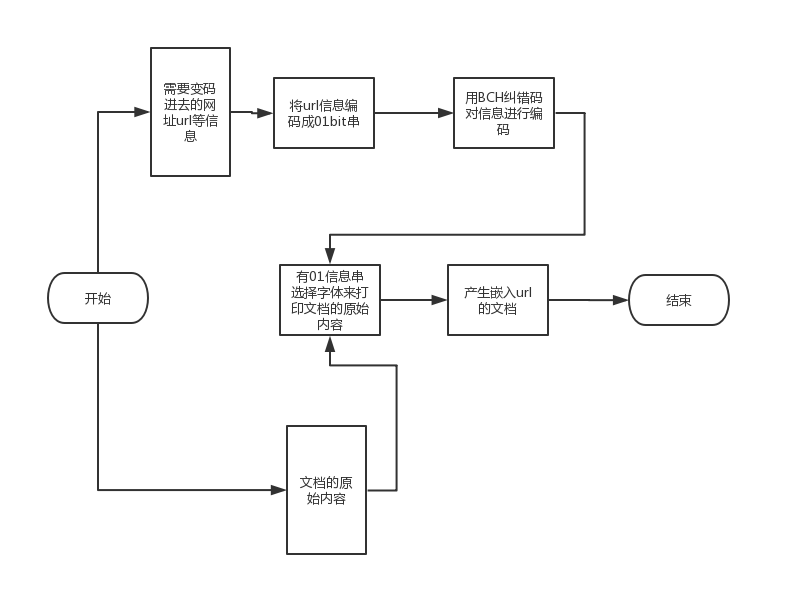
\includegraphics[width=15cm]{figures/generator}
\par\end{centering}
\caption{文档生成流程}

\end{figure}

用户选择需要嵌入的信息(url)和带嵌入的文档内容, 模块对信息(url)进行01编码, 将得到的01bit串进行BCH纠错码编码得到最终的bit串,
文档生成器通过bit串中的0 和1 分别选择两种字体, 按照顺序来生成符合内容的文档.

\subsection{信息恢复模块}

\begin{figure}[H]
\begin{centering}
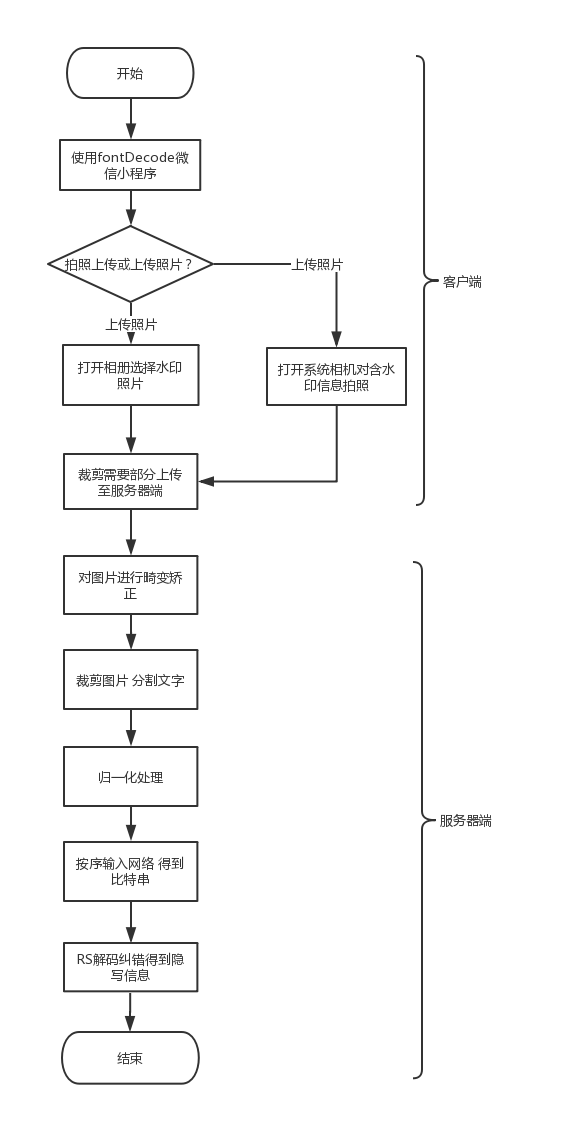
\includegraphics[width=8cm]{figures/recognize-flow-graph}
\par\end{centering}
\caption{信息恢复流程}

\end{figure}

信息恢复模块由客户端和服务器端两部分组成。客户端负责上传含有水印的文档的图片。服务器端负责将客户端上传的图片进行处理,最终将解码所得的隐藏信息返回给客户端。

客户端是一个微信小程序,它能允许用户选择相机拍摄上传或选择相册中图片上传。

服务器端对照片进行畸变校正等预处理, 使得最后的照片能够字体排列整齐, 对矫正过后的图片按照设定的文档规格进行切分, 得到一张张单个字体图片,
将这些单个字体文件按照顺序输入神经网络分类器中进行分类, 按照类别得到01比特串, 输入BCH解码器解码后, 恢复到原有信息。

\section{技术实现}

\subsection{文档生成算法}

\begin{figure}[H]
\begin{centering}
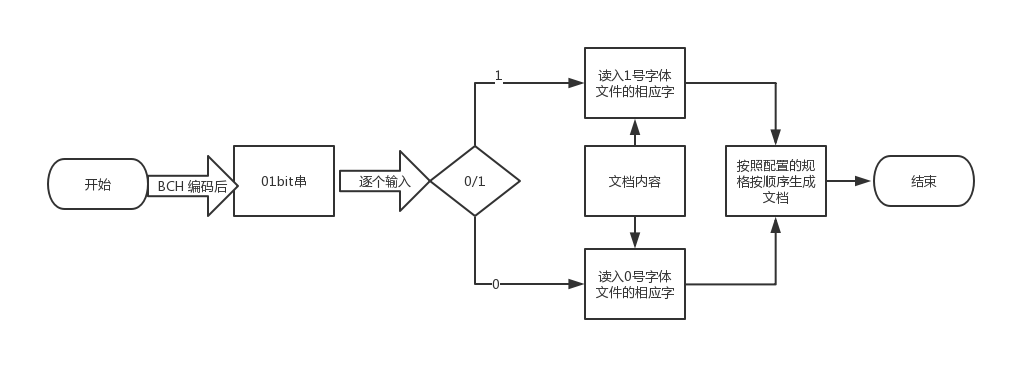
\includegraphics[width=15cm]{figures/doc-gen}
\par\end{centering}
\caption{文档生成算法流程}
\end{figure}

该算法的核心是一个选择生成和doc文档生成器, 这个核心可以根据输入的bit 是0 还是1, 来选择生成文档中对应位置的字使用哪种字体,
0 1bit串输入结束后, 文档文档生成器将结果显示出来, 用户可以选择导出成doc格式和pdf 格式.

\subsection{图像矫正算法}

\begin{figure}[H]
\begin{centering}
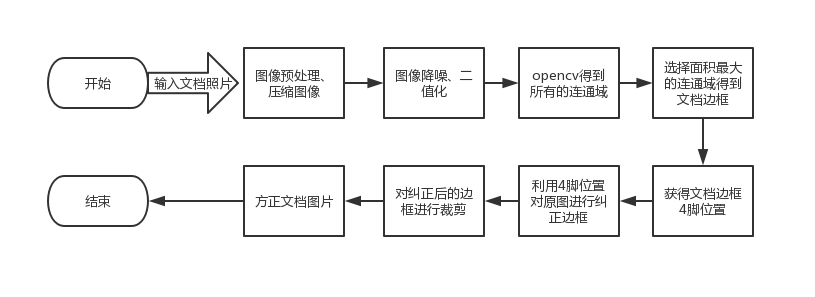
\includegraphics[width=15cm]{figures/image-fix}
\par\end{centering}
\caption{图片矫正算法}
\end{figure}

改算法将输入的照片依次进行如下操作: 图片灰度化, 阈值二值化, 检测轮廓, 寻找轮廓的包围矩阵, 并且获取角度, 根据角度进行旋转矫正,
对旋转后的图像进行轮廓提取, 对轮廓内的图像区域抠出来, 成为一张独立图像. 本算法采用连通域识别的方法, 识别文档照片的边框, 并根据边框的位置进行几何矫正,
最后得到矫正后的图片

\subsubsection{连通域识别}

在图像中,最小的单位是像素,每个像素周围有8个邻接像素,常见的邻接关系有2种:4邻接与8邻接。4邻接一共4个点,即上下左右,如下左图所示。8邻接的点一共有8个,包括了对角线位置的点,如下下图所示。

\begin{figure}[H]
\begin{centering}
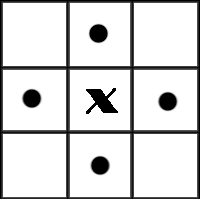
\includegraphics{figures/connectspace1}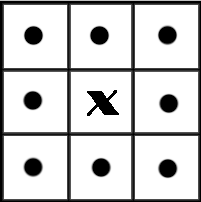
\includegraphics{figures/connectspace2}
\par\end{centering}
\caption{连通域示例}

\end{figure}

如果像素点A与B邻接,我们称A与B连通,于是我们不加证明的有如下的结论: 如果A与B连通,B与C连通,则A与C连通。在视觉上看来,彼此连通的点形成了一个区域,而不连通的点形成了不同的区域。这样的一个所有的点彼此连通点构成的集合,我们称为一个连通区域。下面这符图中,如果考虑4邻接,则有3个连通区域;如果考虑8邻接,则有2个连通区域。(注:图像是被放大的效果,图像正方形实际只有4个像素)。

\begin{figure}[H]
\begin{centering}
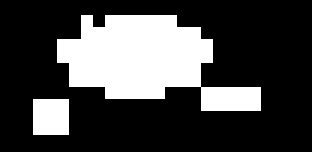
\includegraphics{figures/connectspace3}
\par\end{centering}
\caption{连通域示例}

\end{figure}

连通区域分析是指将图像中的各个连通区域找出并标记。

连通区域分析是一种在CVPR和图像分析处理的众多应用领域中较为常用和基本的方法。例如:OCR识别中字符分割提取(车牌识别、文本识别、字幕识别等)、视觉跟踪中的运动前景目标分割与提取(行人入侵检测、遗留物体检测、基于视觉的车辆检测与跟踪等)、医学图像处理(感兴趣目标区域提取)、等等。也就是说,在需要将前景目标提取出来以便后续进行处理的应用场景中都能够用到连通区域分析方法,通常连通区域分析处理的对象是一张二值化后的图像。

具体的算法如下:
\begin{enumerate}
\item 扫描图像,直到当前像素点B(x,y) == 1:
\begin{enumerate}
\item 将B(x,y)作为种子(像素位置),并赋予其一个label,然后将该种子相邻的所有前景像素都压入栈中;
\item 弹出栈顶像素,赋予其相同的label,然后再将与该栈顶像素相邻的所有前景像素都压入栈中;
\item 重复b步骤,直到栈为空;
\end{enumerate}
此时,便找到了图像B中的一个连通区域,该区域内的像素值被标记为label;
\item (2)重复第(1)步,直到扫描结束;
\item 扫描结束后,就可以得到图像B中所有的连通区域;
\end{enumerate}

\subsubsection{几何校正}

仿射变换和透视变换更直观的叫法可以叫做「平面变换」和「空间变换」或者「二维坐标变换」和「三维坐标变换」,一个是二维坐标(x,y),一个是三维坐标(x,y,z)。也就是:
\begin{enumerate}
\item 仿射变换:

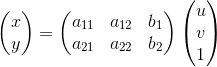
\includegraphics{figures/pasted1}

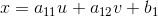
\includegraphics{figures/pasted2}

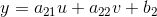
\includegraphics{figures/pasted3}
\item 透视变换:

\paragraph*{\protect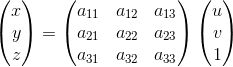
\includegraphics{figures/pasted4}}

\paragraph*{\protect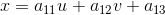
\includegraphics{figures/pasted5}}

\paragraph*{\protect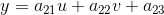
\includegraphics{figures/pasted6}}

\paragraph*{\protect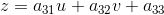
\includegraphics{figures/pasted7}}

\paragraph*{\protect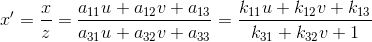
\includegraphics{figures/pasted8}}

\paragraph*{\protect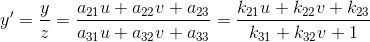
\includegraphics{figures/pasted9}}

\end{enumerate}
摄像机就相当于透视中心,摄像机和荧幕之间就是像点的集合,荧幕上展示的就是目标点集合; 中心点和某一像点的连线和荧幕的交点就是这个像点的目标点;像点(x,
y)和目标点(s, t)是一一对应的关系,我们可以使用一个{[}3x3{]}的矩阵A描述他们之间的映射关系:{[}s, t, 1{]}T
= dot(A, {[}x, y, 1{]}T) -{}-{}- A矩阵乘 (x, y)的齐次坐标的转置就是(s, t)的齐次坐标的转置,每一个透视变换都对应着特定的变换矩阵A

\subsection{字符切割算法}

\begin{figure}[H]
\begin{centering}
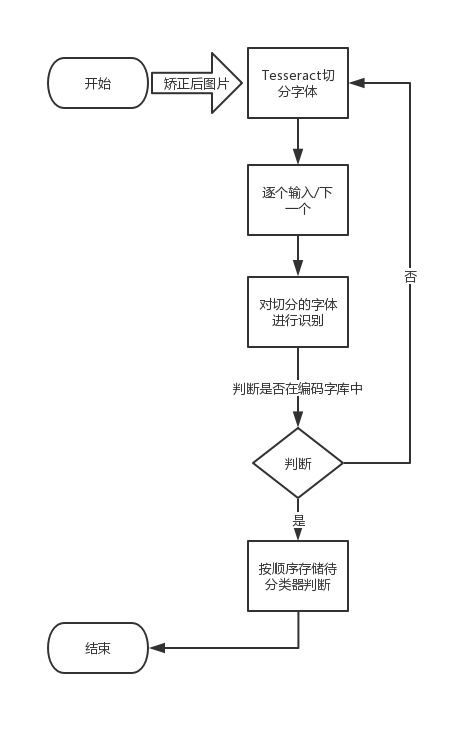
\includegraphics{figures/char-seg}
\par\end{centering}
\caption{字符切分流程}

\end{figure}


\subsubsection{tesseract 介绍}

Tesseract是Ray Smith于1985到1995年间在惠普布里斯托实验室开发的一个OCR引擎,曾经在1995 UNLV精确度测试中名列前茅。但1996年后基本停止了开发。2006年,Google邀请Smith加盟,重启该项目。目前项目的许可证是Apache
2.0。该项目目前支持Windows、Linux和Mac OS 等主流平台。但作为一个引擎,它只提供命令行工具。

\subsubsection{算法过程}

信息恢复模块中, 输入照片校正后, 使用tesseract 对矫正后的照片进行切分, 然后逐个识别, 如果是标点符号则直接丢弃, 如果是中文字,
则识别后判断是否在我们的编码字符库中, 如果不在也丢弃, 最后对切分之后的字符图片按照顺序保存, 待输入到神经网络进行分类和解码.

\subsection{BCH编解码算法}

\begin{figure}[H]
\begin{centering}
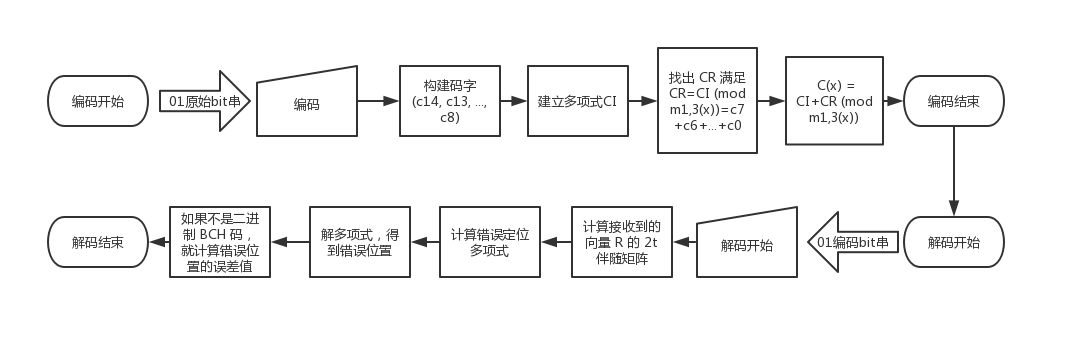
\includegraphics[width=14cm]{figures/bchcodec}
\par\end{centering}
\caption{BCH编解码算法}

\end{figure}


\subsubsection{构建}

BCH 码使用有限域上的域论与多项式。为了检测错误可以构建一个检测多项式,这样接收端就可以检测是否有错误发生。要构建一个能够检测、校正两个错误的
BCH 码,我们要使用有限域 $GF(16)$ 或者 $Z^{2}[x]\lyxmathsym{/}\left(x^{4}+x+1\right)$。如果
$\alpha$ 是 $m_{1}(x)=x^{4}+x+1$ 的一个根,那么 $m_{1}$ 就是 $\alpha$ 的极小多项式,这是因为$m_{1}(x)=(x-\alpha)(x-\alpha^{2})(x-\alpha^{4})(x-\alpha^{8})=x^{4}+x+1$。如果要构建一个能够纠正一个错误的
BCH 码,那么就使用 $m_{1}(x)$,这个代码就是所有满足$C(x)\equiv0\lyxmathsym{(}modm_{1}(x)\lyxmathsym{)}$且根为
$\alpha,\alpha^{2},\alpha^{4},\alpha^{8}$ 的多项式 $C(x)$。

\subsubsection{解码算法}
\begin{enumerate}
\item 首先生成 ${\displaystyle 2t}$ 伴随矩阵 然后生成元素为 ${\displaystyle S_{t\times t}={\begin{bmatrix}s_{1} & s_{2} & s_{3} & ... & s_{t}\\
s_{2} & s_{3} & s_{4}... & ... & s_{t+1}\\
s_{3} & s_{4} & s_{5} & ... & s_{t+2}\\
... & ... & ... & ... & ...\\
s_{t} & s_{t+1} & s_{t+2} & ... & s_{2t-1}
\end{bmatrix}}}\lyxmathsym{的矩阵}{\displaystyle S_{txt}}$
\item 生成元素为 ${\displaystyle C_{t\times1}={\begin{bmatrix}s_{t+1}\\
s_{t+2}\\
...\\
...\\
s_{2t}
\end{bmatrix}}}$ 的矩阵 ${\displaystyle c_{tx1}}$
\item 让 ${\displaystyle \Lambda}\lyxmathsym{表示未知的多项式系数,用}{\displaystyle \Lambda_{t\times1}={\begin{bmatrix}\lambda_{t}\\
\lambda_{t-1}\\
...\\
\lambda_{3}\\
\lambda_{2}\\
\lambda_{1}
\end{bmatrix}}}$表示
\item 这样就得到矩阵方程${\displaystyle S_{t\times t}\Lambda_{t\times1}=C_{t\times1}}$
\item 如果矩阵 ${\displaystyle S_{t\times t}}$存在行列式,那么我们就可以找到这个矩阵的逆,然后就可以得到
${\displaystyle \Lambda}$的值 如果 ${\displaystyle det(S_{t\times t})=0}$,那么按照

\begin{algorithm}[H]
if ${\displaystyle t=0}$

then declare an empty error locator polynomial

stop Peterson procedure.

end

set ${\displaystyle t\leftarrow t-1}$

continue from the beginning of Peterson's decoding
\end{algorithm}

\item 在 ${\displaystyle \Lambda}$的值确定之后,自然就得到错误定位多项式
\item 结束
\end{enumerate}

\subsection{网络模型训练}

\subsubsection{网络结构}

\begin{figure}[H]
\begin{centering}
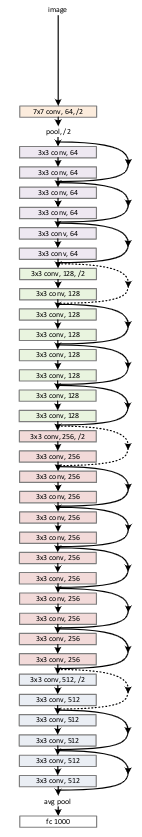
\includegraphics{figures/model}
\par\end{centering}
\caption{神经网络模型}

\end{figure}

使用了类ResBlock 结构, 提高网络的深度和前后连接性来提高分类器的分类能力.

\subsubsection{训练数据}

神经网络的训练需要足量的数据,否则会出现欠拟合(Underfitting)的问题。目前并没有符合本作品需求的中文字体数据集,因此本小组选择自己制造训练和测试用的数据。由于需要多种字体数据进行训练和测试,下面的步骤针对每种字体重复进行:

\paragraph{生成文档}

首先需要批量化地生成“文档”。为了\textbf{简化与关键技术关系不大的部分},本小组使用了简单的规则生成“文档”来解决下述问题,以方便文档矫正和文字切割,针对更复杂的文档格式、布局的处理不在本次作品的研究范围内。
\begin{enumerate}
\item 对于任意指定的文档,从中分割出所有汉字并不容易,因此规定简单文档格式每一页的文字行数、列数固定,且不含非汉字字符,如标点、空格、英文字母等;
\item 文档在屏幕上显示时,边界有时不容易确定,因此在每页文档周边加一个黑色边框;
\item 文档从屏幕或纸张上被拍照后,其页面边界会有一些影响文档边界自动识别的因素,导致边界出现微小偏移,为了降低其对切割出的文字的影响,在文字与文字之间加入一定大小的空白。
\end{enumerate}
下图是一页文档的示例:

\begin{figure}[H]
\begin{centering}
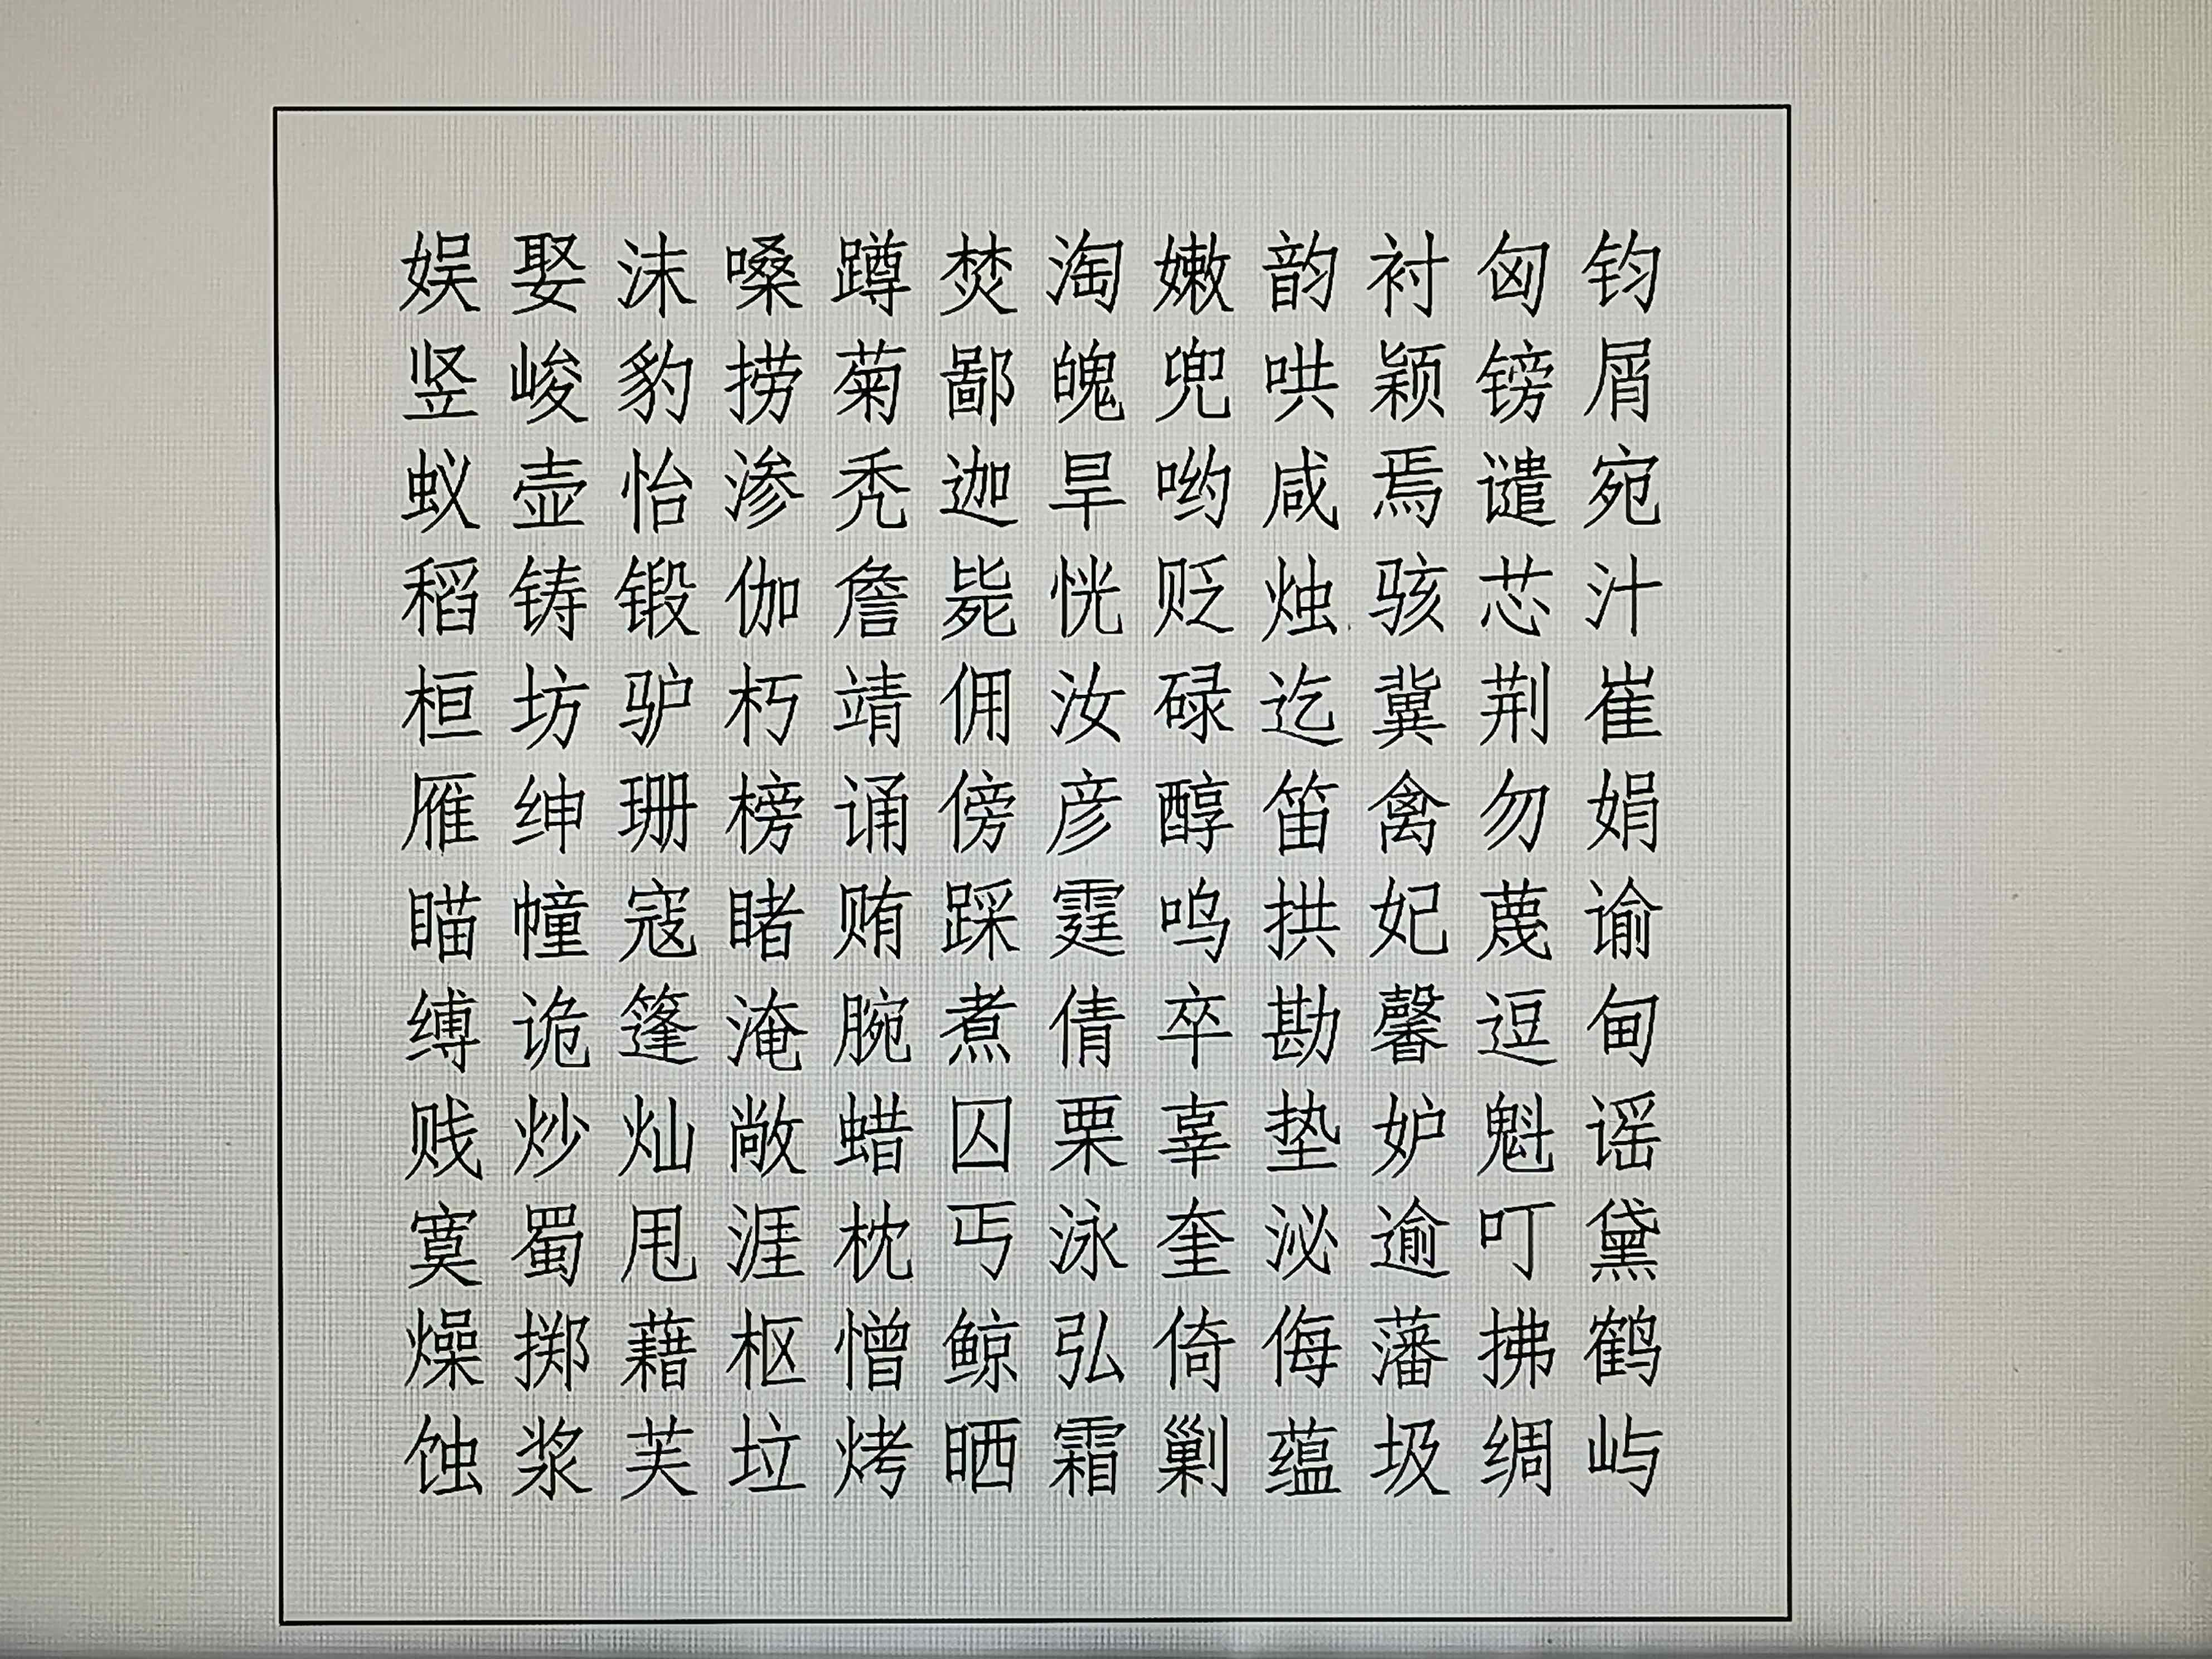
\includegraphics[width=10cm]{figures/before-fix}
\par\end{centering}
\caption{文档示例}
\end{figure}


\paragraph{屏幕拍照}

考虑到用户在拍照时,光照、拍照角度、显示文档的屏幕等因素都很难确定,在制作训练数据时体现出这样的多样性才能使训练出的网络模型具有较好的泛化能力,因此制作训练数据时我们做了以下的变化:
\begin{enumerate}
\item 从多个角度拍照;
\item 变化背景光照、屏幕亮度拍照;
\item 使用不同的屏幕进行拍照;
\item 从不同的距离拍照。
\end{enumerate}

\paragraph{文档矫正}

使用传统算法进行边界识别,然后做透视畸变矫正,得到照片中的文档区域,对于“生成文档”中所示图片,矫正后得到下图:

\begin{figure}[H]
\begin{centering}
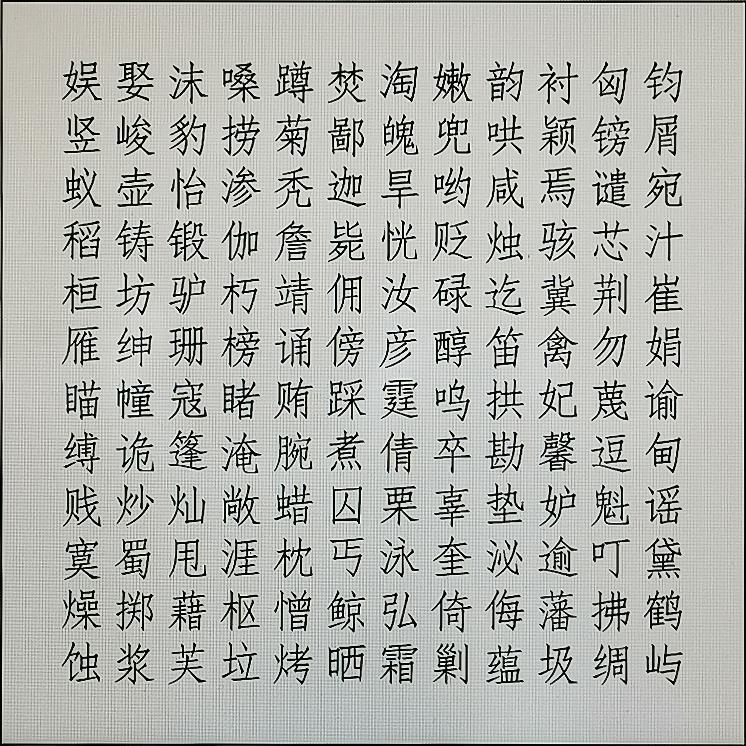
\includegraphics[width=10cm]{figures/after-fix}
\par\end{centering}
\caption{文档示例}
\end{figure}


\paragraph{文字切割}

在矫正后的图像上按照预定的行列数进行均等划分,得到一个一个字的图像。

\section{功能指标}

使用字体识别的准确率来评估本作品的效果。

\newpage{}

\part{作品测试与分析}

原理上本作品可以使用任意多种类的字体作为信息的载体,在本作品的实际实现和测试中,为了突出核心想法,只选择两种字体;为了测试信息恢复的准确性,选择了两种非常相近的字体。其中一种为华文仿宋,另一种
TODO{[}GAN?{]}

\section{测试方案与结果}

我们对本作品的核心功能——信息编码解码,及其周边功能——屏摄文档分割进行测试。

\subsection{单元测试}

\subsubsection{字体人眼不可识别性测试}

作为文档水印,两种编码字体不能被人眼区分是非常重要的。为了确定我们选定字体的差异是否是难以察觉的,我们对一定范围内人群进行了问卷调查。若认为两种字体人肉眼不可区分的人数比到达特定阈值,我们便可以认为选择的两种字体是可以用来编码的。

\subsubsection{字体识别\label{subsec:=005B57=004F53=008BC6=00522B}}

准备一组(超过 200 个)屏摄切割后的文字,识别其字体,计算准确率。准确率计算公式:
\begin{center}
$M=\frac{P_{1}+P_{2}}{T_{1}+T_{2}}$
\par\end{center}

其中 $P_{1}$、$P_{2}$ 为两种字体分别正确识别的数目,$T_{1}$、$T_{2}$为两种字体图片的数目。

屏摄切割后的文字示例如下:

\begin{figure}[H]
\begin{centering}
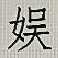
\includegraphics{figures/1}\hspace{1cm}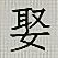
\includegraphics{figures/2}
\par\end{centering}
\medskip{}

\begin{centering}
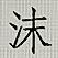
\includegraphics{figures/3}\hspace{1cm}
\includegraphics{figures/4}
\par\end{centering}
\caption{屏摄切割后的文字图像示例}
\end{figure}


\subsubsection{编码解码}

使用随机生成的数据(超过 200 组)进行编码,按照\ref{subsec:=005B57=004F53=008BC6=00522B}中得到的准确率模拟比特翻转,对模拟比特翻转得到的数据进行解码,计算准确率。

\subsubsection{文档分割矫正}

准备一组(超过 20 张)屏摄文档的照片,用我们的文档分割算法进行分割,计算分割的准确率。

\begin{figure}[H]
\begin{centering}
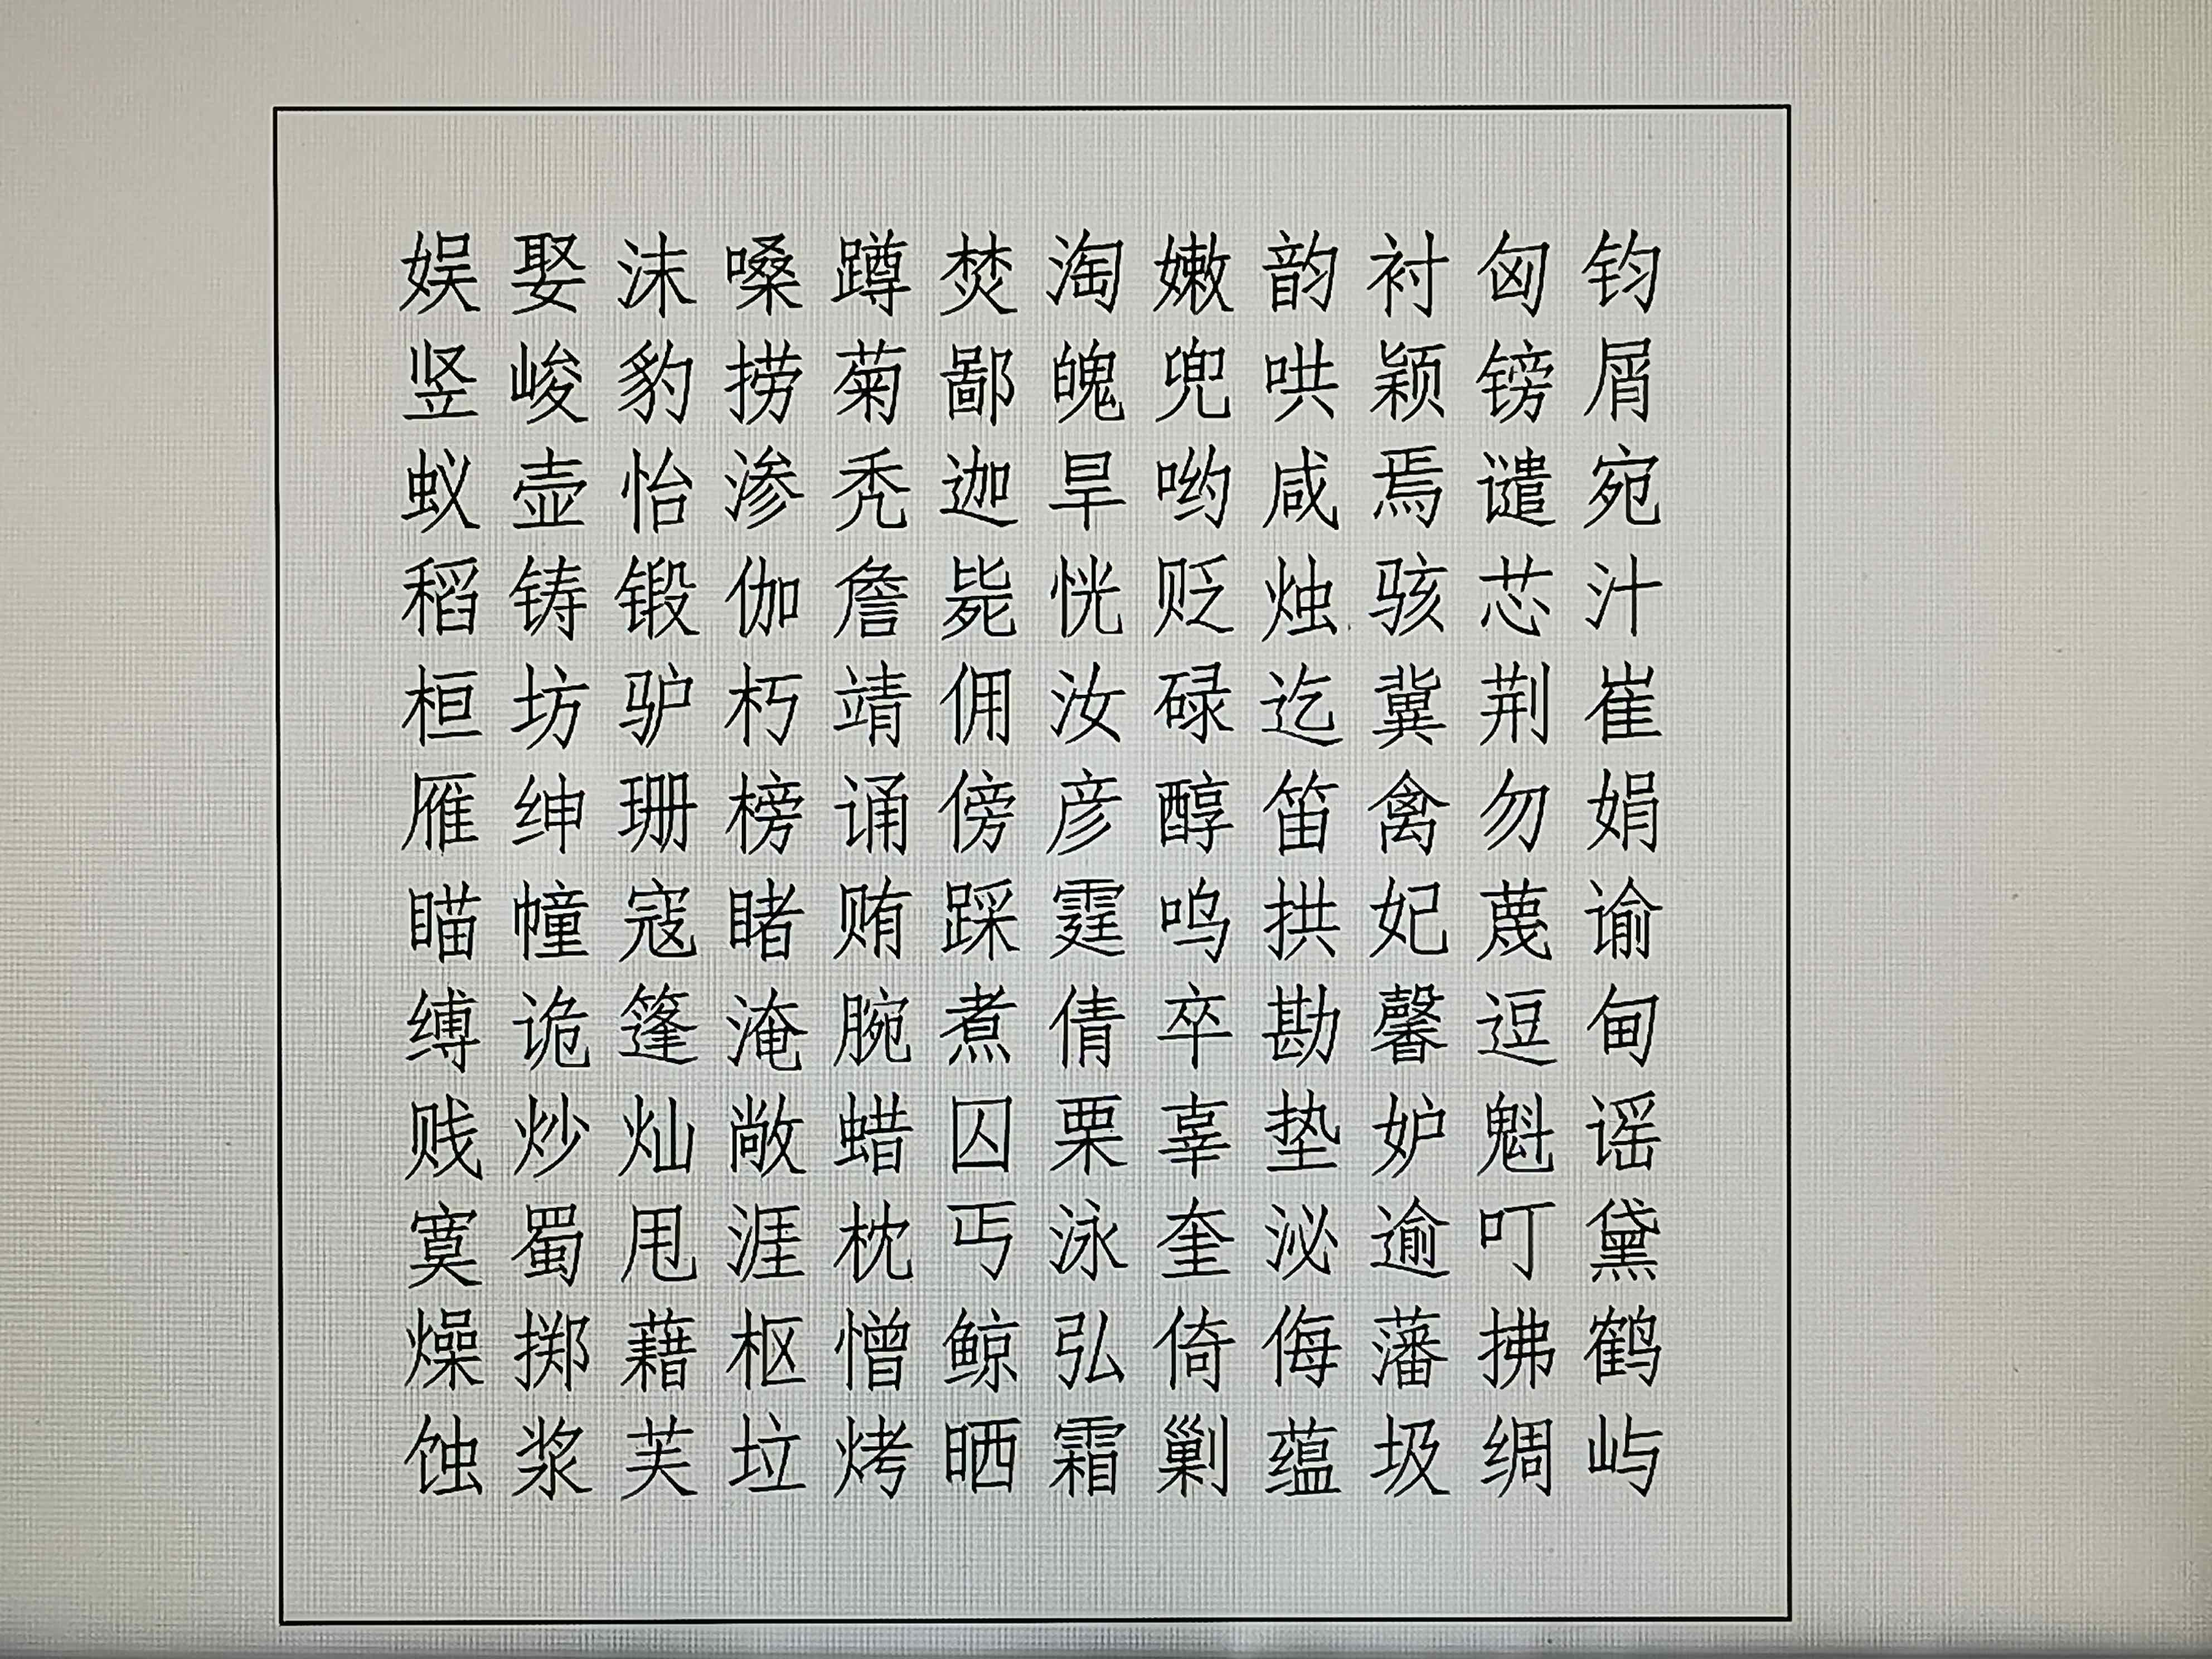
\includegraphics[height=6cm]{figures/before-fix}\hspace*{1cm}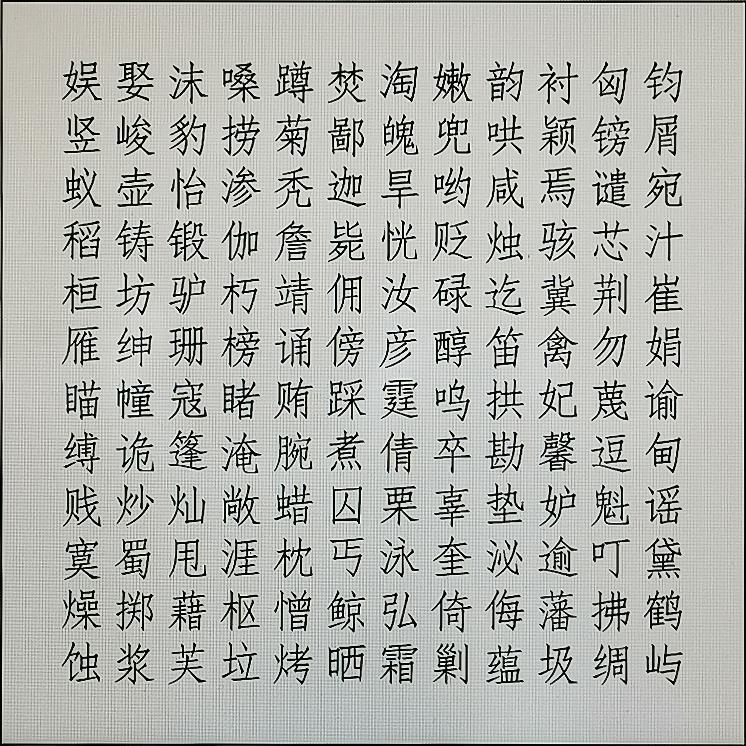
\includegraphics[height=6cm]{figures/after-fix}
\par\end{centering}
\caption{分割前后图像示例}
\end{figure}


\subsection{系统测试}

我们模拟了数次完整的使用流程。先使用给定原始文本和水印内容,使用文档生成模块产生带有水印的文档。再对该文档使用客户端拍照上传,服务器端进行定位、畸变矫正、切字处理后,将字按序输入网络,将输出的比特穿进行BCH解码,就能得到水印信息。下面展示某一次的详细使用流程

\subsubsection{文档生成模块测试}

我们采用\ref{sec:=007279=008272=0063CF=008FF0}中的一段话作为原始文本,'ciscn!'作为待水印信息。将原始文本和给定信息输入文档生成模块,得到的文档如下图所示:

\begin{figure}[H]
\begin{centering}
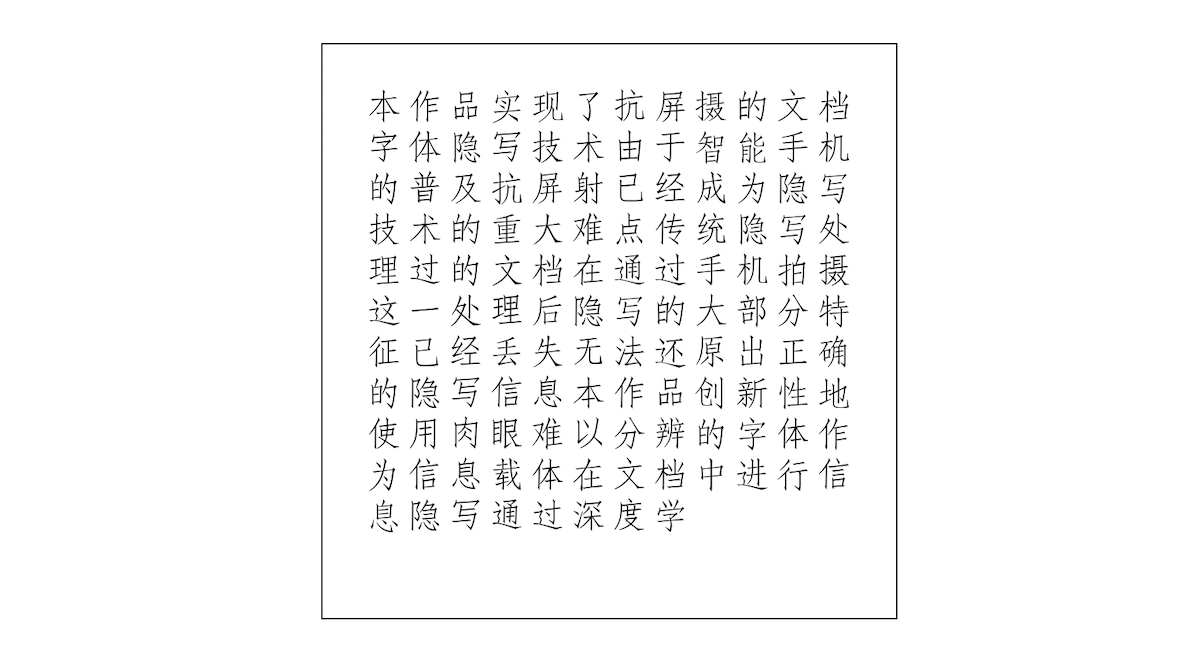
\includegraphics[width=10cm]{figures/system-test/geneate-img}
\par\end{centering}
\centering{}\caption{带有水印的文档}
\end{figure}


\subsubsection{信息恢复模块测试}

打开微信搜索fontDecode小程序,点击中间按钮,你可以选择上传相册中的照片或者临时拍照上传。

\begin{figure}[H]
\begin{centering}
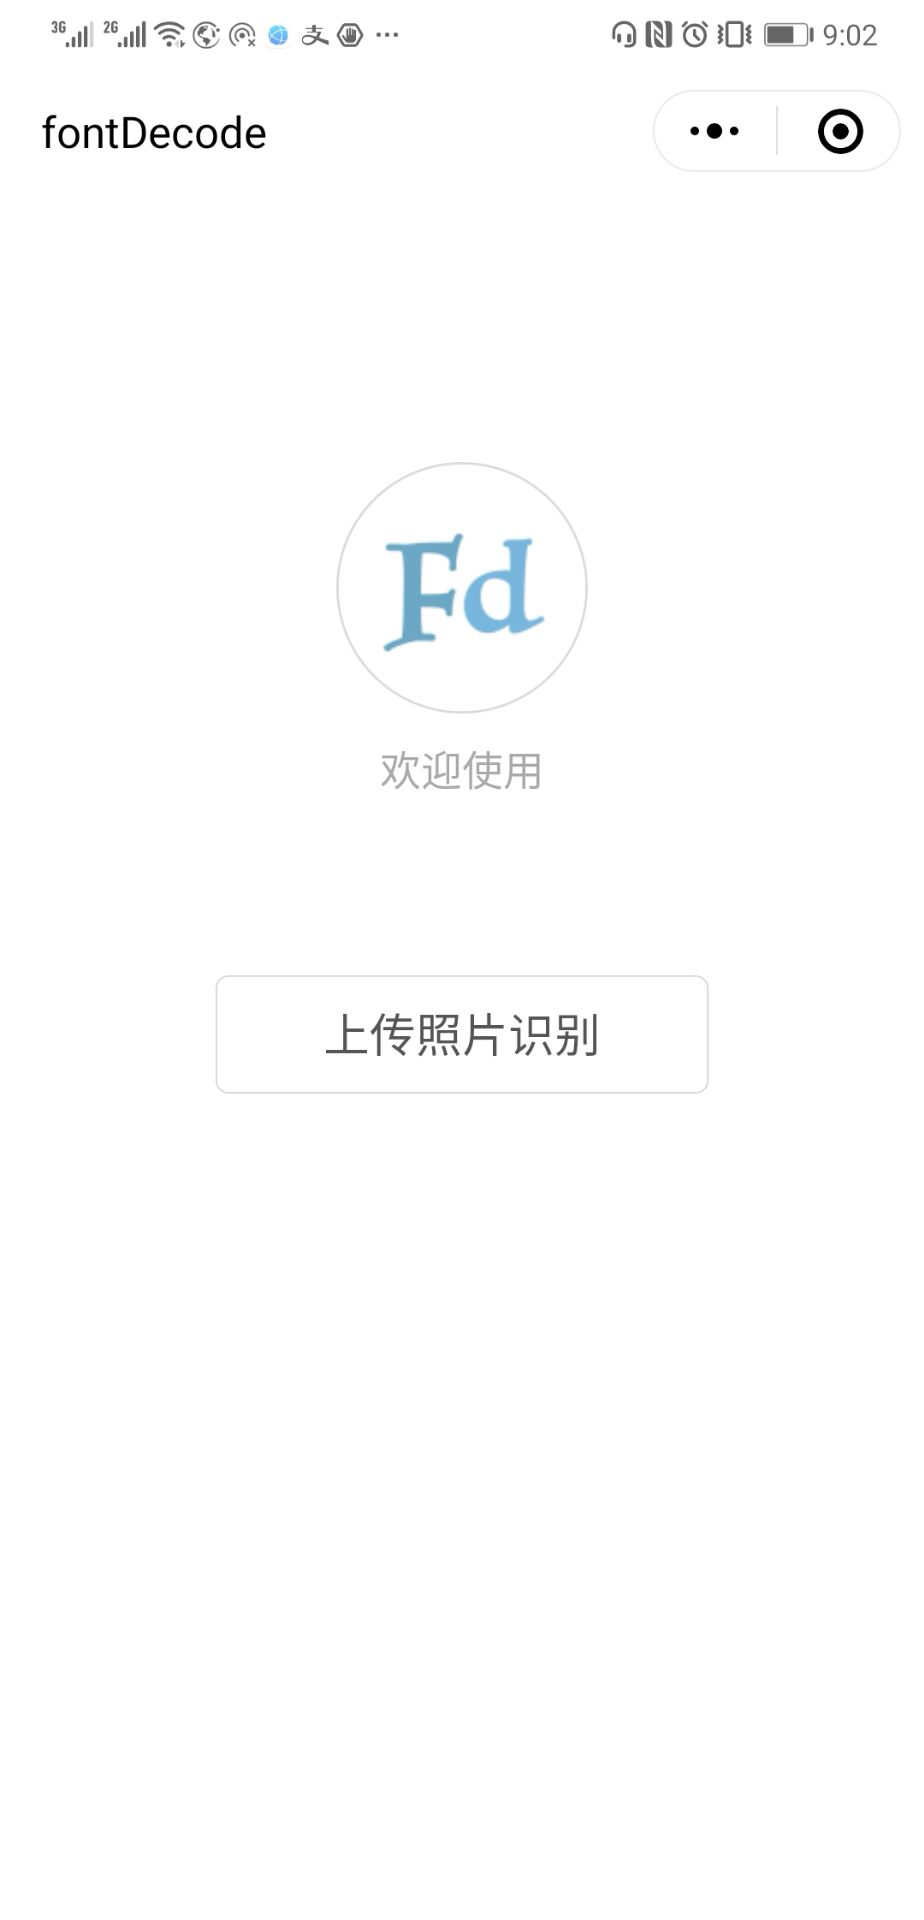
\includegraphics[height=10cm]{figures/system-test/wx-index}\hspace*{2cm}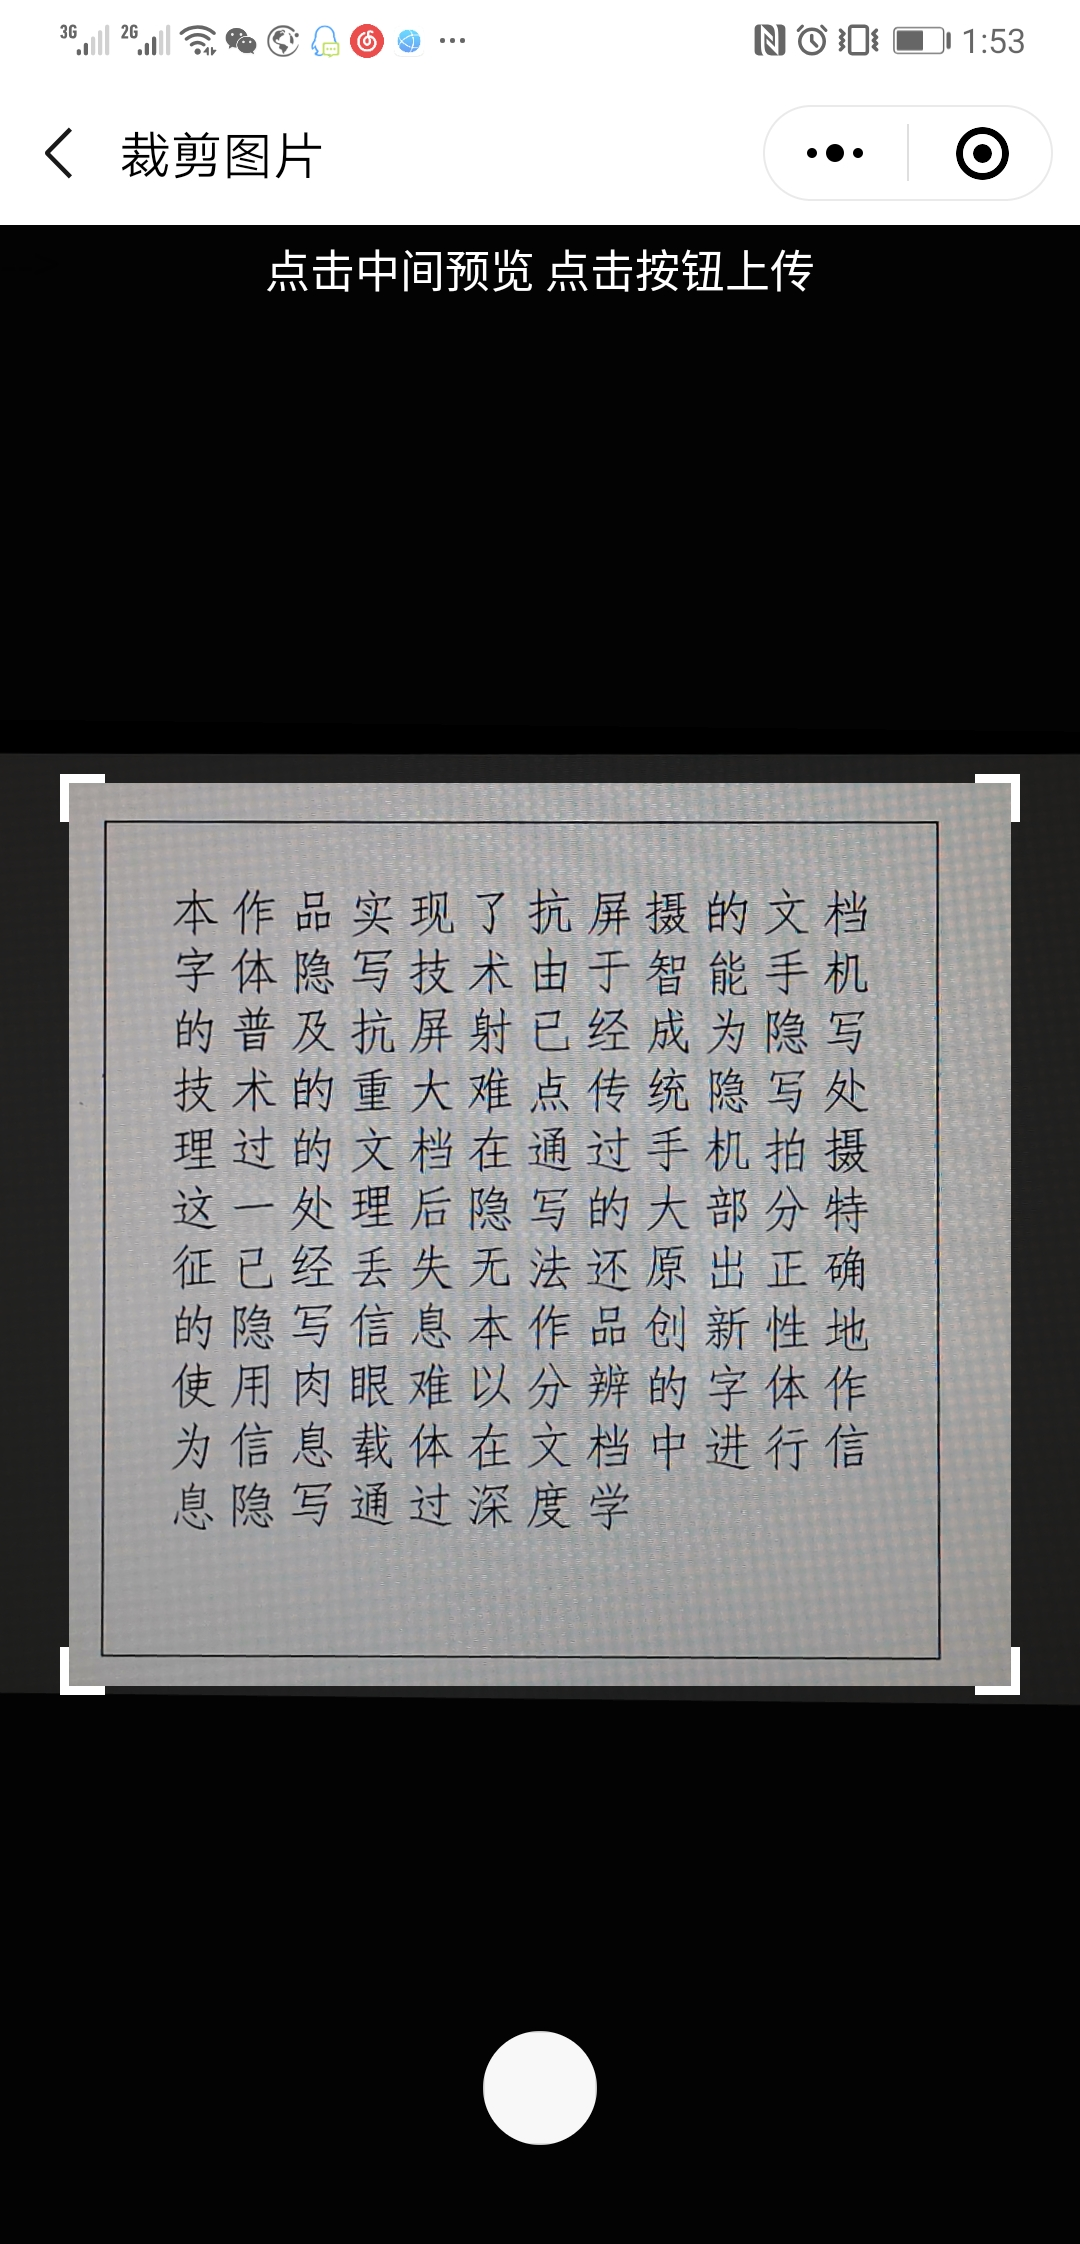
\includegraphics[height=10cm]{figures/system-test/cut-image}
\par\end{centering}
\caption{fontDecode小程序主页 与 裁减页}
\end{figure}

这里我们选择演示拍照上传。打开系统相机后,拍摄屏幕上含有水印的文档(模拟现实拍照场景)。之后,旋转缩放并切割拍到的照片。点击下方按钮将处理后的图片上传至服务器。

服务器收到上传图片后,先进行定位、畸变矫正、切割。将切割后的图片规范到224{*}224并进行归一化处理,依次输入进网络。将网络输出的比特串进行BCH解码,即能得到图片中的隐藏信息。

\begin{figure}[H]
\begin{centering}
\subfloat[服务器畸变矫正后的图像]{\begin{centering}
\includegraphics[width=0.3\linewidth]{figures/system-test/bi\lyxdot \lyxdot \lyxdot }
\par\end{centering}

}\hspace*{2cm}\subfloat[切割后的图像]{\begin{centering}
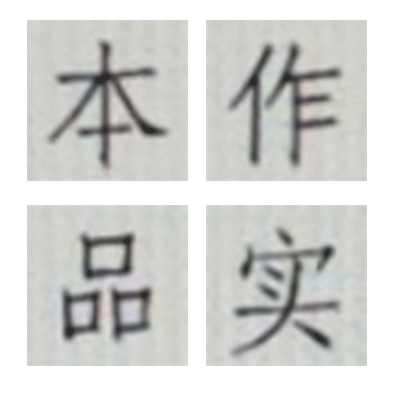
\includegraphics[width=0.25\linewidth]{figures/system-test/cut}
\par\end{centering}

}
\par\end{centering}
\begin{centering}
\caption{服务器端处理}
\par\end{centering}
\end{figure}

之后服务器会将解码得到的信息发回给客户端,用户成功获得隐藏信息。

\begin{figure}[H]
\begin{centering}
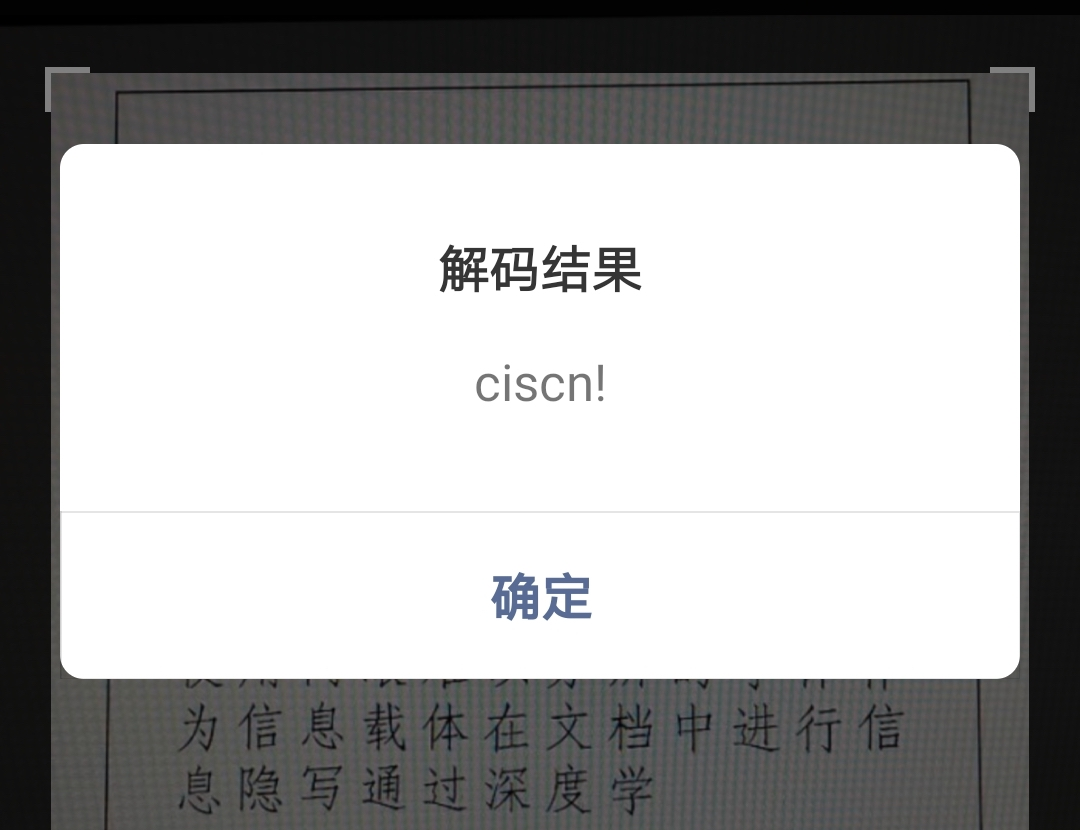
\includegraphics[width=6cm]{figures/system-test/decode-success}
\par\end{centering}
\caption{解码成功截图}
\end{figure}


\section{测试环境}

\subsection{硬件环境}

\paragraph*{移动端}

考虑到微信小程序已具备各手机平台适应性,我们仅选用MI 8、Huawei mate20、360、vivoX7作为移动端测试平台,测试其在微信小程序内打开系统相机、上传图片、裁剪图片和与服务器使用https协议通信的可能性。

不同手机自带的摄像头在性能方面也有不同,如像素值、对焦能力等。因此我们在采集数据时,混合了四款手机拍照得到的照片进行测试训练。增加神经网络对不同手机拍摄出的不同清晰度的图片的识别率。

\paragraph{显示屏}

考虑不同显示屏的分辨率、色差等会对图片产生影响,我们在HP Pavilion 15-au147tx、mac air13.3-inch
(1440 x 900)、mac pro13.3-inch (2560 x 1600)均进行了采样,并在这些显示屏上拍取最终编码后的图片进行解码测试。

\paragraph{服务器端}

服务器端配置为Ubuntu 16.04 64位、1核、内存2G。服务使用nginx+gunicorn+flask进行部署环境。经测试,该环境足够为小量用户提供可靠服务。

\subsection{自然环境}

\paragraph*{光照环境}

光照条件不同对拍照背景颜色有很大影响。在训练网络过程中我们添加了不同光照条件下拍摄的测试集,测试网络对背景颜色的能力。

\paragraph{拍照距离}

由于距离上的差别,拍照所得到的图像在清晰度、摩尔纹等方面有很大的不同。为了测试我们的字体识别网络是否具有处理摩尔纹和清晰度的能力,我们在拍照时随机选取拍照距离。需要注意的是,选取的距离不应过大,使得图片中文字无法识别。也不应过小,使得对整张图片截取不完全,从而无法解码。

\paragraph*{旋转倾斜角度}

为模拟现实情况下拍照环境,我们在拍照时将手机随机进行了小幅度旋转倾斜,以此测试文档分割前图片畸变矫正算法的鲁棒性。

\paragraph{抖动}

测试数据中包含手持拍摄和三脚架固定拍摄数据,以检测网络对模糊图像的识别率。需要注意的是,抖动程度不应太大导致图片文字模糊不清。

\section{结果分析}

TODO

\part{创新性说明}

本作品创新性地将字体作为信息的载体,利用深度学习技术灵活强大的模式识别能力对其进行精准识别,结合纠错编码,在此基础上提出了为文档加水印的技术。

本技术具有如下特点:
\begin{enumerate}
\item 可定制性强\\
原则上,对于任意字体类型、任意字体数目,都可以将本作品提出的技术应用上去。因此本作品提出的水印技术具有很高的可定制性,可以适应于多种场景下文档的字体、水印信息密度等各方面的不同需求,具有广泛的应用价值。
\item 不影响文档的视觉效果\\
目前的实验表明,本作品提出的技术即使使用肉眼难以分辨的字体,字体识别准确率也能够超过 90\%,配合纠错编码,可以以极高的准确率恢复水印信息。因此使用该技术不会给文档带来肉眼可见的变化,这对于文档水印技术是非常重要的。
\item 水印提取准确率高\\
本作品从两个方面提高了水印提取的准确性。一方面,使用字体作为信息载体,文档的水印信息不再容易受到污点、噪点、甚至屏幕拍照出现的摩尔纹的影响;另一方面,深度学习技术使得字体识别更为灵活准确。
\item 去噪能力强\\
在纸质、电子文档的传播过程中可能经过打印、扫描、屏幕显示、拍照等多种变化过程,在这些过程中很容易在文档中留下噪点、污点。传统的分析方法集中于在文档中使用像素点记录信息,很容易受到噪点、污点的影响,导致信息丢失、出错。本作品使用字体作为信息的载体,有效避免了信息被污点、噪点干扰的问题。
\item 信息密度可变\\
虽然在实现和测试时我们只使用了两种字体,但实际上,只要不影响文档阅读效果,可以使用更多字体,从而增加每个文字所能载有的信息量,进而提高同样长度的文档所能包含的信息量,在水印中包含更多信息。
\end{enumerate}

\part{总结}

本作品提出了在中文文档中进行高准确性、高鲁棒性水印的关键技术,并实现了一个原型系统来演示其效果。演示系统基于屏摄文档,但可以扩展到其他形式的文档,具有普遍应用的潜力。

\newpage{}

\bibliographystyle{plain}
\nocite{*}
\bibliography{bib}

\end{document}
